\documentclass{report}
\usepackage{setspace}
\usepackage{graphicx} % Required for inserting images
\usepackage{caption}
\usepackage{subcaption}
\usepackage{amsmath} 
\usepackage[toc,page]{appendix}
\usepackage{adjustbox}
\usepackage{listings}
\usepackage{pgfplots}
\usepackage{makecell}
\usepackage{csvsimple}
\usepackage{physics}
\usepackage{cleveref}
\usepackage[dvipsnames]{xcolor}
%\definecolor{deepgray}{rgb}{.3,.3,.3}
\definecolor{deepblue}{rgb}{0,0,0.5}
\definecolor{deepred}{rgb}{0.6,0,0}
\definecolor{deepgreen}{rgb}{0,0.5,0}
\definecolor{foamC}{rgb}{0,1,1}
\lstset{frame=tb,
        numbers=left,
        basicstyle=\footnotesize\ttfamily,
        keywordstyle=\color{deepblue}\bfseries\ttfamily,
        stringstyle=\color{deepred}\ttfamily,
        commentstyle=\color{deepgreen},%\itshape\ttfamily,
        morecomment=[l][\color{magenta}]{\#},
        showstringspaces=false,
        breaklines=true,
        emphstyle=\bfseries\ttfamily}

\graphicspath{{Figures/}}

\usepackage[		% use biblatex for bibliography
backend=biber,      % use biber or bibtex backend
style=authoryear,   % choose style
natbib=true,		% allow natbib commands
hyperref=true,	    % activate hyperref support
alldates=year,      % only show year (not month)
]{biblatex}

\addbibresource{hw2writeup.bib}

\renewcommand{\chaptername}{Problem}

\title{Homework 3}
\author{Abbie Brunner}
%\date{February 22, 2024}

\onehalfspacing
\begin{document}

\maketitle

\tableofcontents

\chapter{}

\section{Part A}

Given the modified version of Stoke's first problem we are asked to find the equation that governs the x-component of velocity for the fluid above the plate.
The boundary conditions we are given are as follows

\begin{equation*}
   y = 0, \quad \vb{u} = [U, V]
\end{equation*}
\begin{equation*}
   y \rightarrow \infty, \quad \vb{u} \rightarrow [0, 0]
\end{equation*}
\begin{equation*}
   \pdv{x}\qty(\ldots) = 0, \quad \text{\emph{a.k.a.} flow is the same everywhere along the plate}
\end{equation*}

Looking at the x-momentum equation

\begin{equation}
   \pdv{u}{t} + u\pdv{u}{x} + v\pdv{u}{y} = -\frac{1}{\rho}\pdv{P}{x} + \nu\qty(\pdv[2]{u}{x}+\pdv[2]{u}{y})
\end{equation}

We see immediately there are many terms that drop out due to the constant nature along the plate leaving us with

\begin{equation}
   \pdv{u}{t} + v\pdv{u}{y} = \nu\pdv[2]{u}{y}
\end{equation}

\section{Part B}

Here we define $\eta=By/t^n$, $u=t^mAf(\eta)$, and $t^mCg(\eta)$.
We can define derivatives as follows

\begin{equation}
   \pdv{u}{t} = -nmt^{m-1}f'\frac{ABy}{t^{n+1}}
\end{equation}
\begin{equation}
   \pdv{u}{y} = t^mAf'\frac{B}{t^n}
\end{equation}
\begin{equation}
   \pdv[2]{u}{y} = t^m A f'' \frac{B}{t^n}
\end{equation}

We can then plug this in to the x-momentum equation in an attempt to find a similarity solution

\begin{equation}
   \pdv{u}{t}+v\pdv{u}{y} = \nu\pdv[2]{u}{y}
\end{equation}

Plugging this in we find that it reduces to

\begin{equation}
   -nmt^{m-n-2}f'ABy+t^{2m-n}Cgf'B = \nu t^{m-n}Af''B
\end{equation}

From this we see that there is no way to cancel out the time dependence in the equation meaning that there is no similarity solution for this particular configuration.

\chapter{}

In this question we are asked to use a shooting method to numerically solve the Blasius Equation.

\begin{equation}
   f''' + \frac{1}{2}ff''=0
   \label{blas}
\end{equation}
\begin{equation*}
   \text{B.C.s } f'(0) = 0, \quad f(0) = 0, \quad f'(\eta) \rightarrow \text{ as } \eta\rightarrow\infty
   \label{bcs}
\end{equation*}

To do this we can use numeric approximations with a forward differencing scheme.

\begin{equation}
   f'_i = \frac{f_{i+1}-f_i}{\Delta\eta} \quad \Rightarrow \quad f_{i+1} = f_i+\Delta\eta f'_i
   \label{fpdiff}
\end{equation}

We can do similar things for $f''$ and $f'''$, and use \cref{blas} to form the equation to solve for each subsequent $f''$

\begin{equation}
   f''_{i+1} = f''_{i} + \Delta\eta\qty(-\frac{1}{2}f f'')
   \label{shooting}
\end{equation}

Using the provided initial guess of $f''(0) = 0.2$ yields a result of $f'(10) = 0.72479...$, and given the boundary conditions given we know this is not correct.
Massaging the initial guess to a value of $f''(0) = 0.3155$ gives an $f'(10)=1.00624...$, which is significantly closer.
Next we adjust the $\Delta\eta$ in the method going from 0.1 to 0.01.
This is because we are given that the shear is known to be $f''(0) = 0.332$, and reducing the step size allows us to get closer to this value.
Upon changing the $\Delta\eta$ and changing the initial guess to $f''(0) = 0.3305$ leads to the freestream condition of $f'(10)=1.00389...$

\begin{figure}
   \centering
   \makebox[\textwidth][c]{
      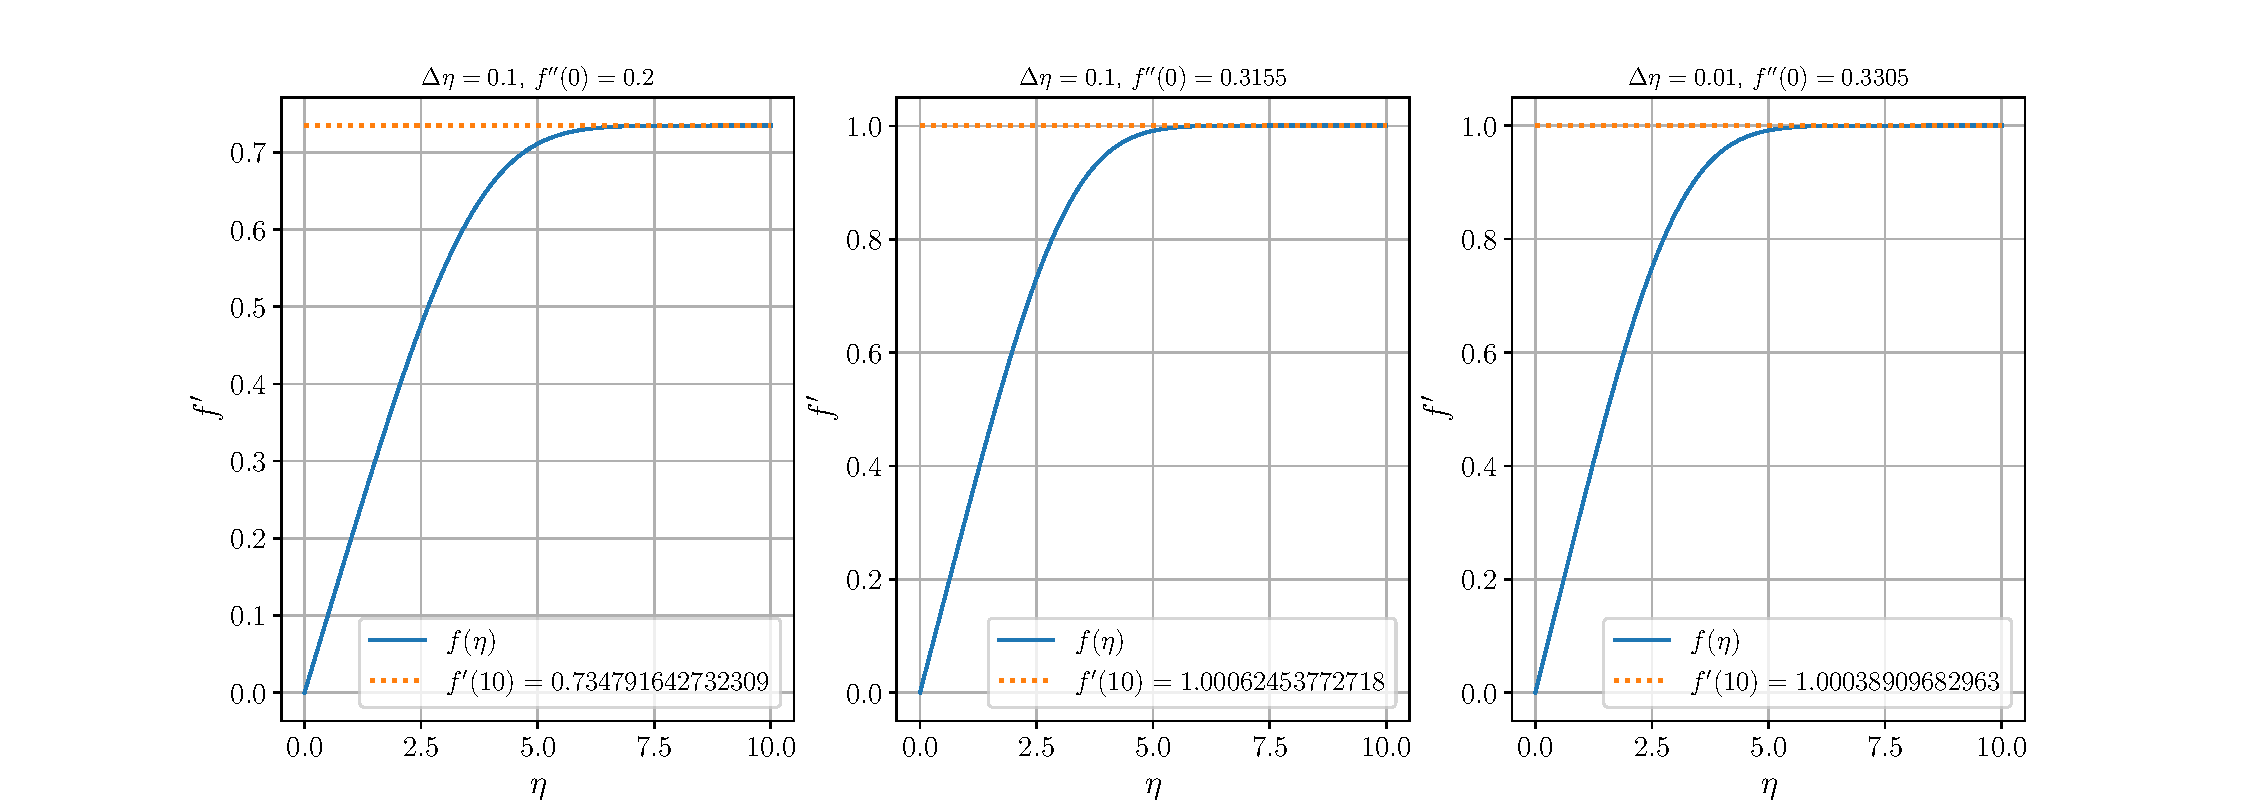
\includegraphics[width=1.5\textwidth]{problem2.pdf}
   }
   \caption{Shooting Method with Three Different Configurations}
   \label{p2g}
\end{figure}

Plots of all three parts are shown in \cref{p2g} and all three show generally the same behavior, but the second and third configurations reflect the B.C.s defined.

\chapter{}

\section{Part A}

\subsection{Parabolic}

We begin by deriving the parabolic approximation of the velocity profile.

\begin{equation}
   \frac{u(y)}{U_{\infty}} = a_0 + a_1\eta + a_2\eta^2 \quad \eta = \frac{y}{\delta}
   \label{parab}
\end{equation}
\begin{equation*}
   \text{B.C.s } u(0) = 0, \quad u(\delta) = U_{\infty}, \quad \eval{\pdv{u}{y}}_{\delta}
\end{equation*}

Applying these boundary conditions shows that $a_0 = 0$.
The rest of the boundary conditions set up the system of equations as shown.

\begin{equation}
   \begin{bmatrix}
      1 & 1 \\
      1 & 2
   \end{bmatrix}
   \begin{bmatrix}
      a_1 \\
      a_2
   \end{bmatrix} =
   \begin{bmatrix}
      1 \\
      0
   \end{bmatrix}
\end{equation}

This can be evaluated to find

\begin{equation}
   \begin{bmatrix}
      a_1 \\
      a_2
   \end{bmatrix}
   =
   \begin{bmatrix}
      2 \\
      1
   \end{bmatrix}
\end{equation}

Thus the parabolic approximation takes the form

\begin{equation}
   \frac{u(y)}{U_{\infty}} = 2\eta - \eta^2
\end{equation}

\subsection{$\order{\eta^3}$ with Wall Boundary condition}

A very similar process can be done for each $\order{\eta^3}$ function, but we will impose different boundary conditions.

\begin{equation}
   \frac{u(y)}{U_{\infty}} = a_0 + a_1\eta + a_2\eta^2 + a_3\eta^3
   \label{parab}
\end{equation}
\begin{equation*}
   \text{B.C.s } u(0) = 0, \quad u(\delta) = U_{\infty}, \quad \eval{\pdv{u}{y}}_{\delta}, \quad \eval{\pdv[2]{u}{y}}_0
\end{equation*}

\begin{equation}
   \begin{bmatrix}
      1 & 1 & 1\\
      1 & 2 & 3 \\
      0 & 2 & 0
   \end{bmatrix}
   \begin{bmatrix}
      a_1 \\
      a_2 \\
      a_3
   \end{bmatrix} =
   \begin{bmatrix}
      1 \\
      0 \\
      0
   \end{bmatrix}
\end{equation}


\begin{equation}
   \begin{bmatrix}
      a_1 \\
      a_2 \\
      a_3
   \end{bmatrix}
   =
   \begin{bmatrix}
      \frac{3}{2} \\
      0 \\
      -\frac{1}{2}
   \end{bmatrix}
\end{equation}

\begin{equation}
   \frac{u(y)}{U_{\infty}} = \frac{3}{2}\eta - \frac{1}{2}\eta^3
\end{equation}

\subsection{$\order{\eta^3}$ with Freestream Boundary Condition}

Finally we impose the final boundary condition where there is zero curvature at $y = \delta$

\begin{equation}
   \frac{u(y)}{U_{\infty}} = a_0 + a_1\eta + a_2\eta^2 + a_3\eta^3
   \label{parab}
\end{equation}
\begin{equation*}
   \text{B.C.s } u(0) = 0, \quad u(\delta) = U_{\infty}, \quad \eval{\pdv{u}{y}}_{\delta}, \quad \eval{\pdv[2]{u}{y}}_{\delta}
\end{equation*}

\begin{equation}
   \begin{bmatrix}
      1 & 1 & 1 \\
      1 & 2 & 3 \\
      0 & 2 & 6
   \end{bmatrix}
   \begin{bmatrix}
      a_1 \\
      a_2 \\
      a_3
   \end{bmatrix} =
   \begin{bmatrix}
      1 \\
      0 \\
      0
   \end{bmatrix}
\end{equation}


\begin{equation}
   \begin{bmatrix}
      a_1 \\
      a_2 \\
      a_3
   \end{bmatrix}
   =
   \begin{bmatrix}
      3 \\
      -3 \\
      1
   \end{bmatrix}
\end{equation}

\begin{equation}
   \frac{u(y)}{U_{\infty}} = 3\eta - 3\eta^2 + \eta^3
\end{equation}

\section{Part B}

Graphing all the results along with our numeric results from Problem 2 yields the results seen in \cref{prob3g}

\begin{figure}
   \centering
   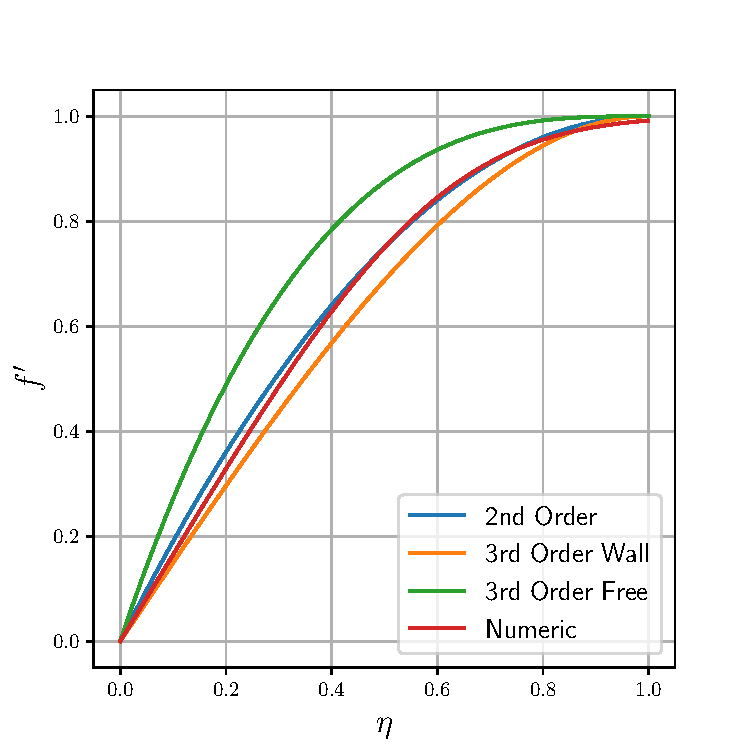
\includegraphics[width=0.5\textwidth]{problem3.pdf}
   \caption{Various Velocity Profiles for Flow Over a Flat Plate}
   \label{prob3g}
\end{figure}

\section{Part C}

The momentum integral equation is as follows

\begin{equation}
   \frac{U_{\infty}\theta}{\nu}\qty[\dv{\theta}{x}+\frac{2\theta+\delta^*}{U_{\infty}}-\frac{V_w}{U_{\infty}} = \frac{\tau_w}{\rho U_{\infty}^2}]
\end{equation}

We can define new variables $H, S, \text{ and }\lambda$ that can be used to scale the momentum integral equation

\begin{equation*}
   H = \frac{\delta^*}{\theta} \quad \lambda = \frac{\theta^2}{\nu}\dv{U_{\infty}}{x} \quad S = \frac{\tau_w\theta}{\mu U_{\infty}}
\end{equation*}

This transforms the MIE to

\begin{equation}
   \frac{U_{\infty}}{2}\dv{x}\qty(\frac{\theta^2}{\nu})+(H+2)\lambda = S
\end{equation}

Following Thwaites' Method to find the momentum thickness as a function of $x$

\begin{equation}
   \theta^2(x) = \frac{0.45\nu}{U^6_{\infty}}\int_{0}^{x} U^5_{\infty} \dd{x}
\end{equation}

For the two third order profiles we can directly compute $\delta^* \text{ and } \theta$ using their respective equations

\begin{equation}
   \delta^* = \int_{0}^{\infty}\qty(1-\frac{u(y)}{U_{\infty}})\dd{y}
\end{equation}

\begin{equation}
   \rho U^2_{\infty} \theta = \rho \int_{0}^{\infty} u(y)\qty(U_{\infty}-u(y)) \dd{y}
\end{equation}

Because $u(\delta) = U_{\infty}$ the integrals go to 0 from $\delta \text{ to } \infty$ and thus we can truncate the integral at $\delta$.
For the first 3rd order approximation this gives us the integrals

\begin{equation}
   \delta^* = \int_{0}^{\delta}\qty(1-\frac{3}{2}\eta+\frac{1}{2}\eta^3)\dd{y}
\end{equation}
\begin{equation}
   \theta = \frac{1}{U_{\infty}}\int_{0}^{\delta}\qty(\frac{3}{2}\eta-\frac{1}{2}\eta^3)\qty(1-\frac{3}{2}\eta-\frac{1}{2}\eta^3)\dd{y}
\end{equation}

Using Wolfram Alpha to solve we get that

\begin{equation}
   \delta^* = \frac{3}{8}\delta \text{ and } \theta = \frac{39}{280}\frac{\delta}{U_{\infty}}
\end{equation}

for the 3rd order approximation with the bounding condition at the wall

Returning to the MIE we see that there is a derivative term of the freestream velocity which is constant.
This then means that this term goes to zero and we are left with

\begin{equation}
   \dv{\theta}{x} = \frac{C_f}{2}
\end{equation}

We also know that

\begin{equation}
   \frac{C_f}{2} = \frac{\tau_w}{\rho U^2_{\infty}}
\end{equation}

Shear stress is defined as

\begin{equation}
   \tau_w = \eval{\mu\pdv{u}{y}}_{y=0} = \mu \eval{\qty(\frac{3}{2}\frac{1}{\delta}-\frac{3}{2}\frac{y^2}{\delta^3})}_{y=0} = \mu \frac{3}{2} \frac{1}{\delta}
\end{equation}

Thus $\theta$ can be computed as follows

\begin{equation}
   \dv{\theta}{x} = \frac{1}{\rho U^2_{\infty}}\qty(\frac{3\mu}{2\delta})
\end{equation}
\begin{equation}
   \theta(x) = \frac{3\nu}{2\delta U^2_{\infty}}x
\end{equation}

The second equation with the bounding condition at the edge of the boundary layer is solved similarly with the integrals

\begin{equation}
   \int_{0}^{\delta}\qty(1-\qty(3\eta-3\eta^2+\eta^3))\dd{y}
\end{equation}
\begin{equation}
   \theta = \frac{1}{U_{\infty}}\int_{0}^{\delta}\qty(3\eta-3\eta^2+\eta^3)\qty(1-\qty(3\eta-3\eta^2+\eta^3))\dd{y}
\end{equation}

which can once again be solved to find that

\begin{equation}
   \delta^* = \frac{\delta}{4} \quad \theta = \frac{3}{28}\delta
\end{equation}

The shear stress for this approximation can be solved as follows

\begin{equation}
   \tau_w = \eval{\mu\pdv{u}{y}}_{y=0} = \mu \eval{\qty(3\frac{1}{\delta}-6\frac{y}{\delta^2}+3\frac{y^2}{\delta^3})}_{y=0} = 3\mu\frac{1}{\delta}
\end{equation}

\section{Part D}

Both third order profiles deviate from the numeric solution more than the parabolic solution.
The third order scheme with the wall boundary condition trends towards a slightly more adverse pressure gradient than the numeric solution.
The other third order scheme deviates more with a pressure gradient that is more favorable than reality.


\end{document}
